% Overview of section
In the previous section, we described how \code{rfactor} transforms a Halide reduction to expose new data parallelism. Doing so requires synthesizing the associative binary operator equivalent to the Halide \emph{update} definition being factored. In this section we describe how we do this synthesis.

% Set up problem, LUT solution
In some cases generating the equivalent associative operator from an update definition is trivial (e.g.\ summation). In other cases it is not, especially when the function reduces onto multiple values (see the examples in Figure~\ref{fig:subgraphs}). The \emph{inverse} problem is easier: Given an associative binary operator, it is straightforward to generate the Halide update definition that implements reduction by it. Therefore, if there were a \emph{small} finite set of associative binary operators, we could simply attempt to match the update definition being factored against each of them in turn. Halide already includes facilities for doing regex-like matching of expressions against patterns with wildcards. Unfortunately, there are more meaningful associative binary operators than could reasonably be thought of ahead of time by a compiler author.

% Full synthesis solution
An alternative approach is to use program synthesis techniques~\cite{Solar-Lezama:2008:PSS:1714168, Torlak:2013:GSL:2509578.2509586} to synthesize the corresponding associative reduction at compile-time when the call to \code{rfactor} is made. This is intractably slow, and can increase compile times of Halide pipelines from seconds to hours.

% Our solution
We use a hybrid of the two approaches, amplified with a strategy for decomposing each synthesis problem into several simpler problems. The overall strategy is shown in Figure~\ref{fig:system}.  Offline, we generate a large finite table of one- and two-dimensional \emph{elementary} associative binary operators and their identities. These are akin to primes -- they are the associative operators which cannot be decomposed into a combination of simpler associative binary operators. The table also contains flags that indicate if the operators are also commutative. At compile-time, we decompose the given Halide update definition into a composition of simpler, lower-dimensional definitions in the same way, then search the table for the elementary operator corresponding to each. If consistent matches are found, we reassemble the results into a composite associative operator equivalent to the original update definition. In Section~\ref{subsec:generation} we describe how we generate the table, and in Section~\ref{subsec:decomposition} we describe the decomposition procedure.

\begin{figure}[tb]
\centering
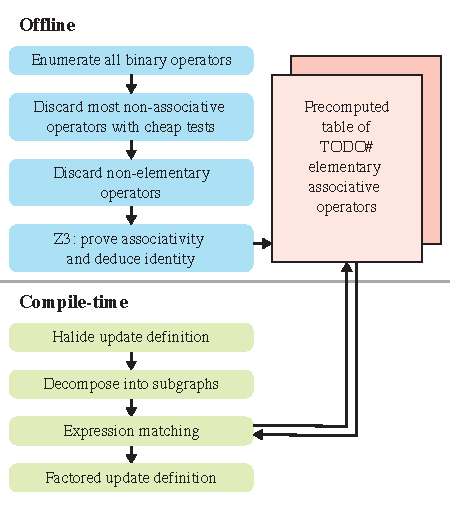
\includegraphics[width=3.2in]{system}
\caption{To factor a reduction written as a Halide update definition, we must first synthesize the equivalent associative binary operator. We generate a large table of elementary associative operators offline by enumerating all non-trivial expression trees and filtering out the ones that are not associative operators. At compile-time, we then decompose the given update definition into simpler definitions and match each against the table. Combining the results gives us the equivalent associative binary operator, which we can use to generate the factored form of the reduction.}
\label{fig:system}
\end{figure}



\subsection{Generating Elementary Operators}
\label{subsec:generation}

We begin with an enumeration of all one- and two-dimensional tuples of expression trees in two tuple inputs $x$ and $y$. The operators used to form the inner nodes of the trees are Halide's IR nodes (\code{*}, \code{+}, \code{-}, \code{min}, \code{max}, \code{select}, \code{<}, etc). We can reject some classes of uninteresting expressions by excluding them from the enumeration altogether.

\begin{enumerate}
\item We only generate trees which use both $x$ and $y$.
\item During matching we canonicalize both the pattern and the input expression using the Halide simplifier and solver; thus, we can make the enumeration more tractable by only generating trees that are already in canonical form.  The canonicalization strategy moves all instances of a variable in an expression tree as far to the left and as far up the tree as possible. We canonicalize expressions to the following form: wherever possible, $x_i$ is to the left of $x_{i+1}$ and any $y_j$ is to the left of $y_{j+1}$. Constants are always on the right.
\item We generate trees using a single generic constant $k$, rather than generating trees containing all possible constants as leaves.
\item We do not generate trees that would be trivially simplified. For example, we do not generate subexpressions like $max(x_0, x_0)$.
\end{enumerate}

After generating a large set of candidate expressions in this manner, we then subject the expressions to a battery of tests so that only elementary associative operators remain. The tests are arranged in increasing order of expense, so that we can cheaply reject most expressions.

\begin{enumerate}
\item For an operator $f$, we construct the expressions $f(f(x, y), z)$ and $f(x, f(y, z))$, and substitute in 100 randomly-selected values for $x, y, z, k$. If the two expressions don't evaluate to the same thing, the expression is not associative and can be rejected.
\item We then reject operators which can be decomposed using the decomposition procedure in Subsection~\ref{subsec:decomposition}.
\item Finally, to \emph{prove} that the expression is associative, we use the Z3~\cite{DeMoura:2008:ZES:1792734.1792766} SMT solver to verify that $\forall x, y, z, k \;f(f(x, y), z) = f(x, f(y, z))$, where $k$ is the constant contained within the function $f$. If this proof succeeds, we then ask Z3 to solve\\ $\forall x, k \;f(id, x) = x$ to synthesize the identity $id$ and to decide its commutativity. This commutativity flag is used to determine the validity of calling \code{rfactor} on the inner loop dimensions of an associative reduction.
\end{enumerate}

In the table of expressions that this produces, $x$ represents the partial result being reduced onto, and $y$ is a wildcard which could match any expression. When matching, $x$ must also appear on the left-hand-side of the update definition. $y$ may depend on the reduction domain coordinates, but may not depend on the partial results. The constant $k$, if it exists, may match anything which neither depends on the reduction domain coordinates nor the partial result. For example, the update definition which separately computes the sum-of-squares of the even and odd values of some input \code{in} could be written as:

\code{f(in(r)\&1) = f(in(r)\&1) + in(r)*in(r)}

\noindent This would match against the pattern $x = x + y$, where $x$ matches \code{f(in(r)\&1)}, and $y$ matches \code{in(r)*in(r)}.

We terminate the enumeration at trees with 8 leaves for the purposes of the experiments described in this work. Since some operations are associative in certain scalar types and not others, we generate different tables for each of Halide's scalar types.  This takes 1.5 days and generates around 9,000 elementary operators to match against per type. Many of the operators are simple operators written in a complex way: as we wish to catch all ways in which a programmer might write a reduction, we make no attempt to exclude these from the table. For faster retrieval, the table of each Halide's scalar type is split into subtables based on the root IR node (e.g. \code{Add}, \code{Mul}, etc.) of the expression. Within each subtable, the operators are ordered based on the total number of leaves (simple expressions are located at the top of the table since they are more likely to be encountered in practice). The operators we use are \code{Add}, \code{Sub}, \code{Mul}, \code{Min}, \code{Max}, comparisons, and \code{Select} (Halide’s if-then-else construct). We then linearly scan the sub-table searching for a matching expression. The first 10 elementary associative operators for signed 32-bit integers are shown in Listing~\ref{fig:top10}.

\begin{figure}
\centering
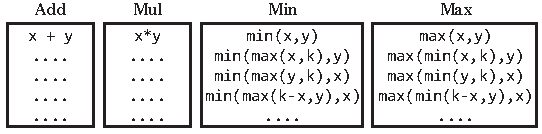
\includegraphics[width=\columnwidth]{tables}
\caption{The first 10 elementary associative operators for 32-bit signed integers organized into subtables based on the root IR node, with simpler expressions located at the top. The boolean flag on the left indicates the commutativity of the expression.}
\label{fig:top10}
\end{figure}

%\begin{lstlisting}[float,caption={The first 10 elementary associative operators for 32-bit signed integers}, label={lst:top10}]
%x + y
%x * y
%min(x, y)
%max(x, y)
%max(min(x, k), y)
%min(max(x, k), y)
%max(min(y, k), x)
%min(max(y, k), x)
%max(min(k - x, y), x)
%min(max(k - x, y), x)
%\end{lstlisting}

%As the list grows, operators become more and more esoteric. An example 8-leaf operator from the list for unsigned integers is TODO

As we only consider one- and two-dimensional expressions, there are meaningful primitive operators that we never discover. For example, we never generate quaternion multiplication, since it is an elementary associative operator in 4 tuple elements, where every expression tree has 8 leaf nodes. We must add any important higher-dimensional primitive operators to our table manually.

%Another limitation is that for each associative reduction, we have a single pattern for the update definition we expect to see, and so if the Halide simplifier and solver fail to canonicalize an update definition into that form, we will not recognize it. For example, consider the reduction which counts how many points in the reduction domain satisfy some predicate $P$. It may be written with the addition outermost:

%\code{f() = select(P(r), 1, 0) + f()}

%After canonicalization we recognize this as a sum reduction of the form \code{x = x + y}. One might also write it with the \code{select} outermost:

%\code{f() = select(P(r), f() + 1, f())},

%We do not recognize this as a sum reduction.

\begin{figure}[tb]
\centering
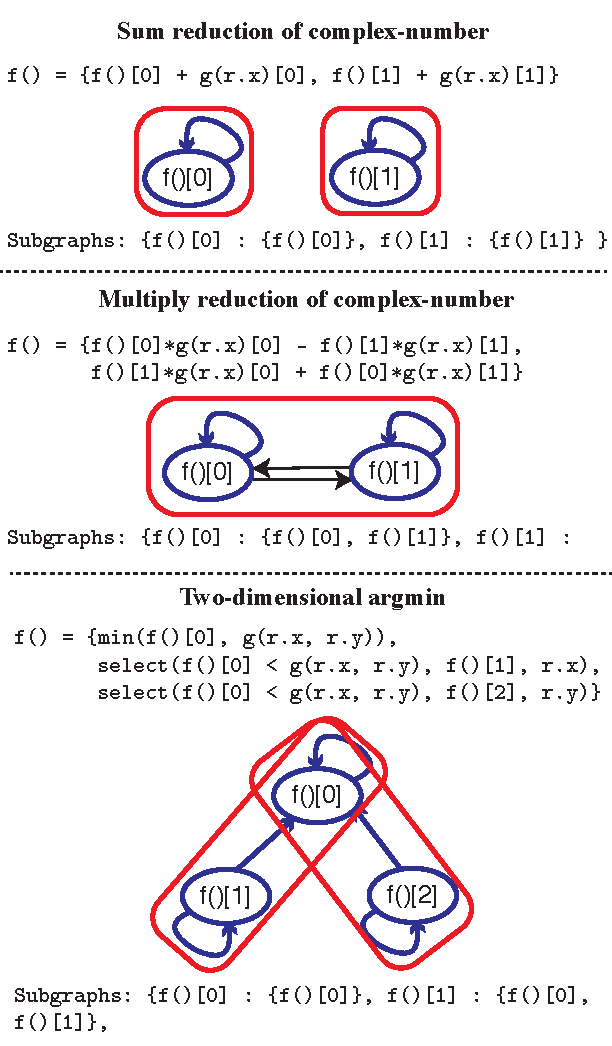
\includegraphics{subgraphs}
\caption{Dependency graphs of various multi-valued Halide \emph{update} definitions. Their subgraph decompositions are shown in red dotted circle. To find the associative operator equivalent to a complex Halide update definition, we first decompose it into subgraphs, then search for each subgraph in our precomputed table of elementary operators, then recompose the results into a single multi-valued associative operator.}
\label{fig:subgraphs}
\end{figure}

\subsection{Subgraph Decomposition}
\label{subsec:decomposition}

To describe how we decompose reductions into elementary operators, we must first discuss how one might \emph{compose} elementary reductions. The simplest way to compose two reductions into a higher-dimensional reduction is to compute them at the same time, independently. This means that reductions that are a concatenation of smaller independent associative reductions are also associative. For example, the tuple computation:

\code{f() = \{f()[0] + in(r), f()[1] * in(r)\}}

is associative, because it is a composition of the following two associative reductions:

\code{f0() = f0() + in(r)}

\code{f1() = f1() * in(r)}

Secondly, if we have an associative operator in which two tuple elements compute the same value, we can deduplicate it, reducing the dimensionality by one. The result is still associative. Therefore, we can prove a reduction is associative by duplicating one of the elements to break a dependency and then applying the rule above. Consider the case of two-dimensional \code{argmin}:

\begin{lstlisting}
f() = {
  min(f()[0], in(r.x, r.y)),
  select(f()[0] < in(r.x, r.y), f()[1], r.x),
  select(f()[0] < in(r.x, r.y), f()[2], r.y)}
\end{lstlisting}

The three tuple elements are the minimum value, and its $x$ and $y$ coordinate. All three tuple elements depend on the minimum value \code{f()[0]}, so we cannot decompose this into independent reductions immediately. Let us duplicate the first tuple element to break the dependency:

\begin{lstlisting}
f() = {
  min(f()[0], in(r.x, r.y)),
  select(f()[0] < in(r.x, r.y), f()[1], r.x),
  min(f()[2], in(r.x, r.y)),
  select(f()[2] < in(r.x, r.y), f()[3], r.y)}
\end{lstlisting}

There are now no dependencies between the first two elements and the last two. This is a simple concatenation of two single-variable \code{argmin} operations. Single-variable \code{argmin} uses two tuple elements, and is present in our table of primitive operators, so we recognize two-dimensional \code{argmin} as associative via its decomposition into two one-dimensional \code{argmin} reductions.

In general we consider the directed graph of dependencies between tuple elements. There is a vertex per tuple element, and an edge from vertex $i$ to vertex $j$ whenever the definition of tuple element $i$ refers to tuple element $j$. If we repeatedly duplicate vertices (tuple elements) to break dependencies, in the limit the graph has one connected component per original tuple element, and that component is the subgraph containing the vertices reachable from that tuple element. If each such subgraph is an associative reduction, then the original reduction is associative. See Figure~\ref{fig:subgraphs} for several examples.

%The general way to apply these two rules to decompose an arbitrary reduction into its components is to construct the directed graph $G$ of dependencies between tuple elements. There is a vertex $N_i$ for each tuple element $i$, and there is an edge from $N_i$ to $N_j$ whenever the value of tuple element $i$ depends on tuple element $j$. The two rules above can then be stated as:

%\begin{enumerate}
%\item If every connected component of $G$ is an associative reduction, then $G$ is an associative reduction.
%\item If we duplicate one of the nodes of $G$, partitioning its incoming edges arbitrarily between the two copies, then the resulting graph is associative iff $G$ is associative, as they compute the same thing.
%\end{enumerate}

% This is a shitty ``proof''
%Let the subgraph $S_i$ be all vertices and edges reachable from $N_i$. We can make a copy of $S_i$ as its own connnected component set apart from the rest of $G$ by the following procedure: Initialize $S_i$ to contain only a duplicate of $N_i$, with no incoming edges. Then repeatedly consider all edges that leave $S_i$, and make duplicates of the vertices they point to, where edges from vertices within $S_i$ point to the duplicate, and edges from vertices not in $S_i$ point to the original. This procedure terminates when $S_i$ contains all vertices reachable from $N_i$. At that point, there are no edges between $S_i$ and the rest of $G$, so it is its own connected component. Once we construct each such $S_i$, we can discard $G$, as everything it computes is also computed by one of the disconnected subgraphs. Similarly, we can discard subgraphs which are completely contained by some other subgraph. Therefore, if every subgraph $S_i$ not contained within some other subgraph is an associative reduction, then $G$ is an associative reduction. For examples of these graphs and their subgraphs for several reductions see Figure \ref{fig:subgraph}.

% Merging results of decomposition
After finding the associative operator equivalent to each subgraph separately, we need to combine the results into a single multi-valued associative operator equivalent to the entire update definition. If all the subgraphs are associative and have identities, we need to ensure that for each tuple element appearing in multiple subgraphs, the binary associative operators deduced via each subgraph are all the same in that tuple element. If they are consistent, we have succeeded in finding an equivalent multi-valued associative operator for the update definition.

In some cases, this procedure over-partitions the graph. We are searching for an associative operator in $x$ and $y$. Only the $x$ is apparent from the Halide update definition -- it is the term that also appears on the left-hand-side. If we decompose based on cross-dependencies within $x$ alone we will miss dependencies between tuple elements that exist only in $y$. Consider 2x2 matrix multiplication written as a four-dimensional reduction:

\begin{lstlisting}
f() = {f()[0] * in(r)[0]) + f()[1] * in(r)[2]),
       f()[0] * in(r)[1]) + f()[1] * in(r)[3]),
       f()[2] * in(r)[0]) + f()[3] * in(r)[2]),
       f()[2] * in(r)[1]) + f()[3] * in(r)[3])}
\end{lstlisting}

Decomposition based on $x$ alone (i.e. \code{f()[i]}) results in 2 subgraphs: one containing the 1st and 2nd tuple elements and one containing the 3rd and 4th tuple elements. Including $y$ (i.e. \code{in(r)[i]}) tells us that the two subgraphs are indeed connected. Therefore, if we fail to find a match for the initial subgraphs (the ones decomposed based on $x$ only), we need to consider other possible grouping of those initial subgraphs. The total number of possible grouping is the Bell number of the initial number of subgraphs. However, we only need to consider grouping expressions which share a common subexpression, and we do not need to consider groups of size greater than the maximum tuple size in our precomputed table. If we do not find a matching associative operator under all possible groupings of the initial subgraphs, we terminate and return an error.

\subsection{Algorithm Summary}
\label{subsec:algorithm}

To summarize, synthesizing an equivalent binary associative operator from a Halide reduction involves the following steps:
\begin{enumerate}
 	\item Starting from the right-hand-side of the update definition, replace all references to the partial results being reduced onto with the symbol $x_i$ where $0 \le i < n$ and $n$ is the number of components in the reduction (i.e. the tuple size).
        \item Canonicalize these expressions. Wherever possible, $x_i$ is to the left of $x_{i+1}$ and constants to the right.
        \item Construct the graph $G$ that represents the dependency relationships between these terms.
        \item Decompose $G$ into an initial set of connected subgraphs $S_0$.
	\item Pick a grouping $S$ from all possible groupings of $S_0$ (see Section \ref{subsec:decomposition}). For the first iteration, we pick $S = S_0$ as the grouping. \label{list:restart_decompose}
	\item For each subgraph in $S$, search the appropriate subtable (based on the data type and root IR node) for a matching associative operator via wildcard matching. If any of the subgraphs are not found, return to step \ref{list:restart_decompose}.
	\item Combine the results into a single multi-valued associative operator equivalent to the entire reduction. If the results are consistent (see Section \ref{subsec:decomposition}), we have found an equivalent associative operator; otherwise, return to step \ref{list:restart_decompose}. If we do not find a matching associative operator after exhausting all possible groupings, we terminate and return an error.
\end{enumerate}
As we show in the next section, this algorithm is fast to execute at compile-time, and successfully finds equivalent binary associative operators for many Halide reductions.
